\documentclass[../psets.tex]{subfiles}

\pagestyle{main}
\renewcommand{\leftmark}{Problem Set \thesection}
\setcounter{section}{6}
\setenumerate[1]{label={\textbf{\arabic*.}}}
\setenumerate[2]{label={(\arabic*)}}

\begin{document}




\section{Nonlinear Stability}
\subsection*{Problems Related to Fundamental Definitions}
\begin{enumerate}
    \item \marginnote{12/2:}Consider the planar system
    \begin{equation*}
        \begin{pmatrix}
            x\\
            y\\
        \end{pmatrix}'
        =
        \begin{pmatrix}
            -x\\
            x^2+y\\
        \end{pmatrix}
    \end{equation*}
    \begin{enumerate}
        \item Find the explicit expression of the flow $\phi_t(z,w)$ and determine the stable and unstable manifolds of the fixed point $(0,0)$. Sketch the phase portrait.
        \begin{proof}
            First off, note that the initial condition is $(z,w)^T$. From the first coordinate IVP, we have the general solution
            \begin{equation*}
                x' = -x
                ,\quad
                x(0) = z
                \quad\Longleftrightarrow\quad
                x(t) = z\e[-t]
            \end{equation*}
            Using this result, we can solve the second coordinate IVP using the Duhamel formula, as follows.
            \begin{equation*}
                y' = (1)y+z^2\e[-2t]
                ,\quad
                y(0) = w
                \quad\Longleftrightarrow\quad
                y(t) = w\e[t]+\int_0^t\e[t-\tau]z^2\e[-2\tau]\dd\tau
            \end{equation*}
            Simplifying the above and combining the results yields the following explicit expression for the flow.
            \begin{equation*}
                \boxed{
                    \phi_t
                    \begin{pmatrix}
                        z\\
                        w\\
                    \end{pmatrix}
                    =
                    \begin{pmatrix}
                        z\e[-t]\\
                        w\e[t]-\frac{z^2\e[t](\e[-3t]-1)}{3}\\
                    \end{pmatrix}
                }
            \end{equation*}
            The stable manifold is the set of all points $x$ such that $\phi_t(x)\to 0$ as $t\to +\infty$. Evaluating componentwise, we see from the first component $x(t)=z\e[-t]$ that $z$ can take any value and we will still have $x(t)\to 0$ as $t\to +\infty$. Note that $w$ can also take on any value without affecting the convergence of $x(t)$. Thus, the first component does not yield any constraints.\par
            The second component, on the other hand, does. Rewrite the expression and regroup the terms to all those of the form $\e[at]$ where $a>0$ and all those $\e[at]$ where $a<0$.
            \begin{align*}
                y(t) &= w\e[t]-\frac{z^2}{3}\e[-2t]+\frac{z^2}{3}\e[t]\\
                &= \left[ w+\frac{z^2}{3} \right]\e[t]+\left[ -\frac{z^3}{3} \right]\e[-2t]
            \end{align*}
            Thus, to get convergence of the above term, we must have
            \begin{align*}
                w+\frac{z^2}{3} &= 0\\
                w &= -\frac{z^2}{3}
            \end{align*}
            $z$ can still take on any value.\par
            Therefore,
            \begin{equation*}
                \boxed{W_s(0) = \left\{ \left( z,-\frac{z^2}{3} \right) \,\middle|\, z\in\R \right\}}
            \end{equation*}
            We can derive the solution for the unstable manifold similarly. This time, we want $\phi_t(x)\to 0$ as $t\to -\infty$. From the first component, we can see that the only case in which $x(t)=z\e[-t]\to 0$ as $t\to -\infty$ is if $z=0$. We don't have any constraints on $w$ from the first component.\par
            With $z=0$, the second component becomes $y(t)=w\e[t]$. This will converge to 0 as $t\to -\infty$ for any $w$.\par
            Therefore,
            \begin{equation*}
                \boxed{W_u(0) = \{(0,w)\mid w\in\R\}}
            \end{equation*}
            i.e., the unstable manifold is the $y$-axis.\par
            Sketching the phase portrait gives something like this:
            \begin{center}
                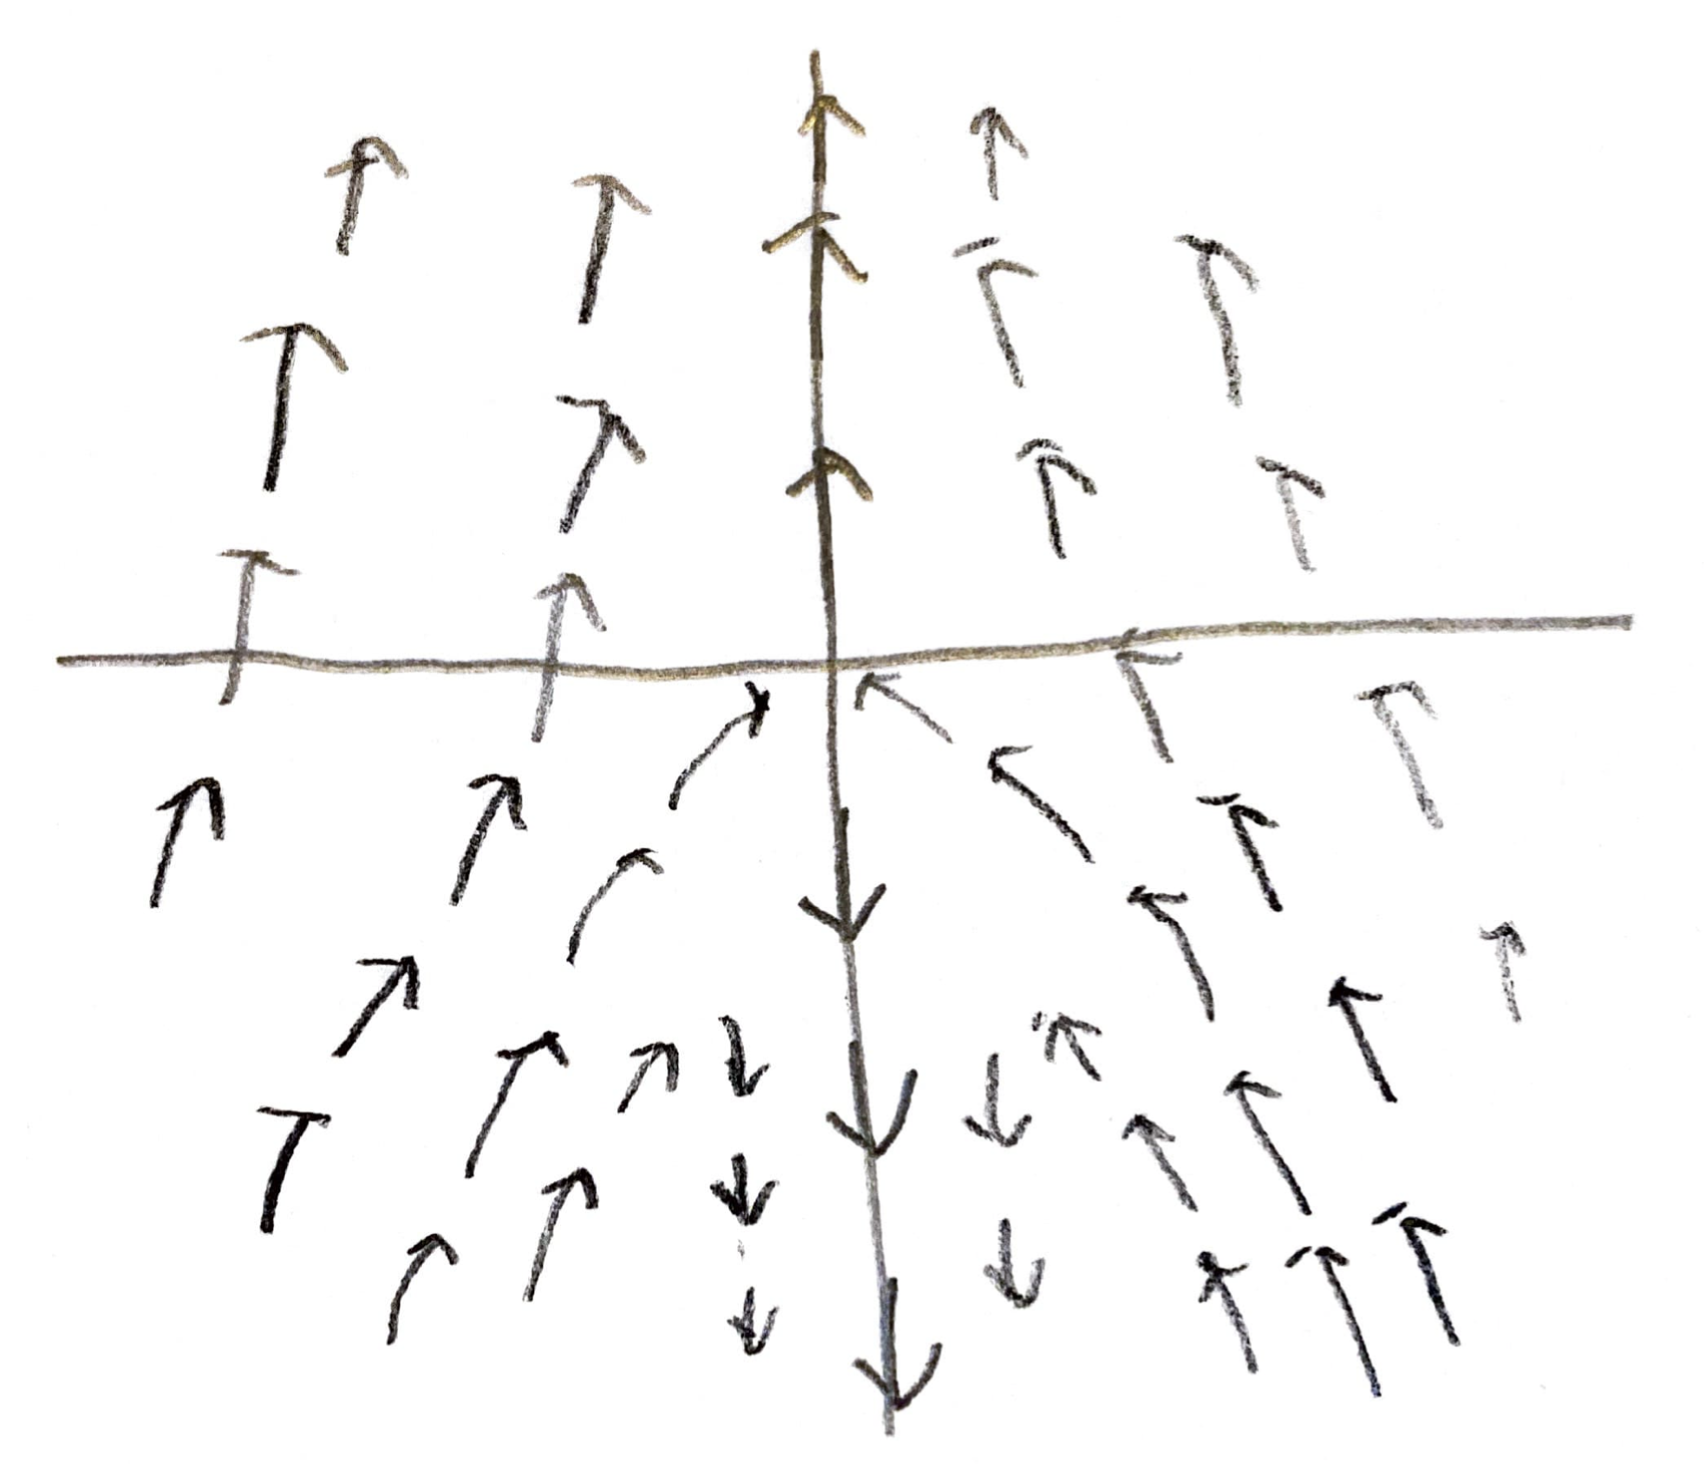
\includegraphics[width=0.4\linewidth]{../ExtFiles/pset7_1-1.png}
            \end{center}
        \end{proof}
        \item Pretend that you do not know how to solve the system, and compute the flow of the linearized system, together with the stable and unstable subspaces. Sketch the phase portrait.
        \begin{proof}
            The Jacobian at 0 is
            \begin{equation*}
                A =
                \begin{pmatrix}
                    -1 & 0\\
                    0 & 1\\
                \end{pmatrix}
            \end{equation*}
            Thus, the flow of the linearized system is
            \begin{align*}
                \phi_t
                \begin{pmatrix}
                    z\\
                    w\\
                \end{pmatrix}
                &= \e[tA]
                \begin{pmatrix}
                    z\\
                    w\\
                \end{pmatrix}\\
                &=
                \begin{pmatrix}
                    \e[-t] & 0\\
                    0 & \e[t]\\
                \end{pmatrix}
                \begin{pmatrix}
                    z\\
                    w\\
                \end{pmatrix}\\
                \Aboxed{
                    \phi_t{
                        \begin{pmatrix}
                            z\\
                            w\\
                        \end{pmatrix}
                    }
                    &= z\e[-t]{
                        \begin{pmatrix}
                            1\\
                            0\\
                        \end{pmatrix}
                    }+w\e[t]{
                        \begin{pmatrix}
                            0\\
                            1\\
                        \end{pmatrix}
                    }
                }
            \end{align*}
            The eigenvalues and eigenvectors are
            \begin{align*}
                \lambda_1 &= 1&
                    \lambda_2 &= -1\\
                v_1 &=
                \begin{pmatrix}
                    0\\
                    1\\
                \end{pmatrix}&
                    v_2 &=
                    \begin{pmatrix}
                        1\\
                        0\\
                    \end{pmatrix}
            \end{align*}
            so the stable subspace is the \fbox{$x$-axis} ($\spn(v_2)$) and the unstable subspace is the \fbox{$y$-axis} ($\spn(v_1)$).\par
            Sketching the phase portrait gives something like this:
            \begin{center}
                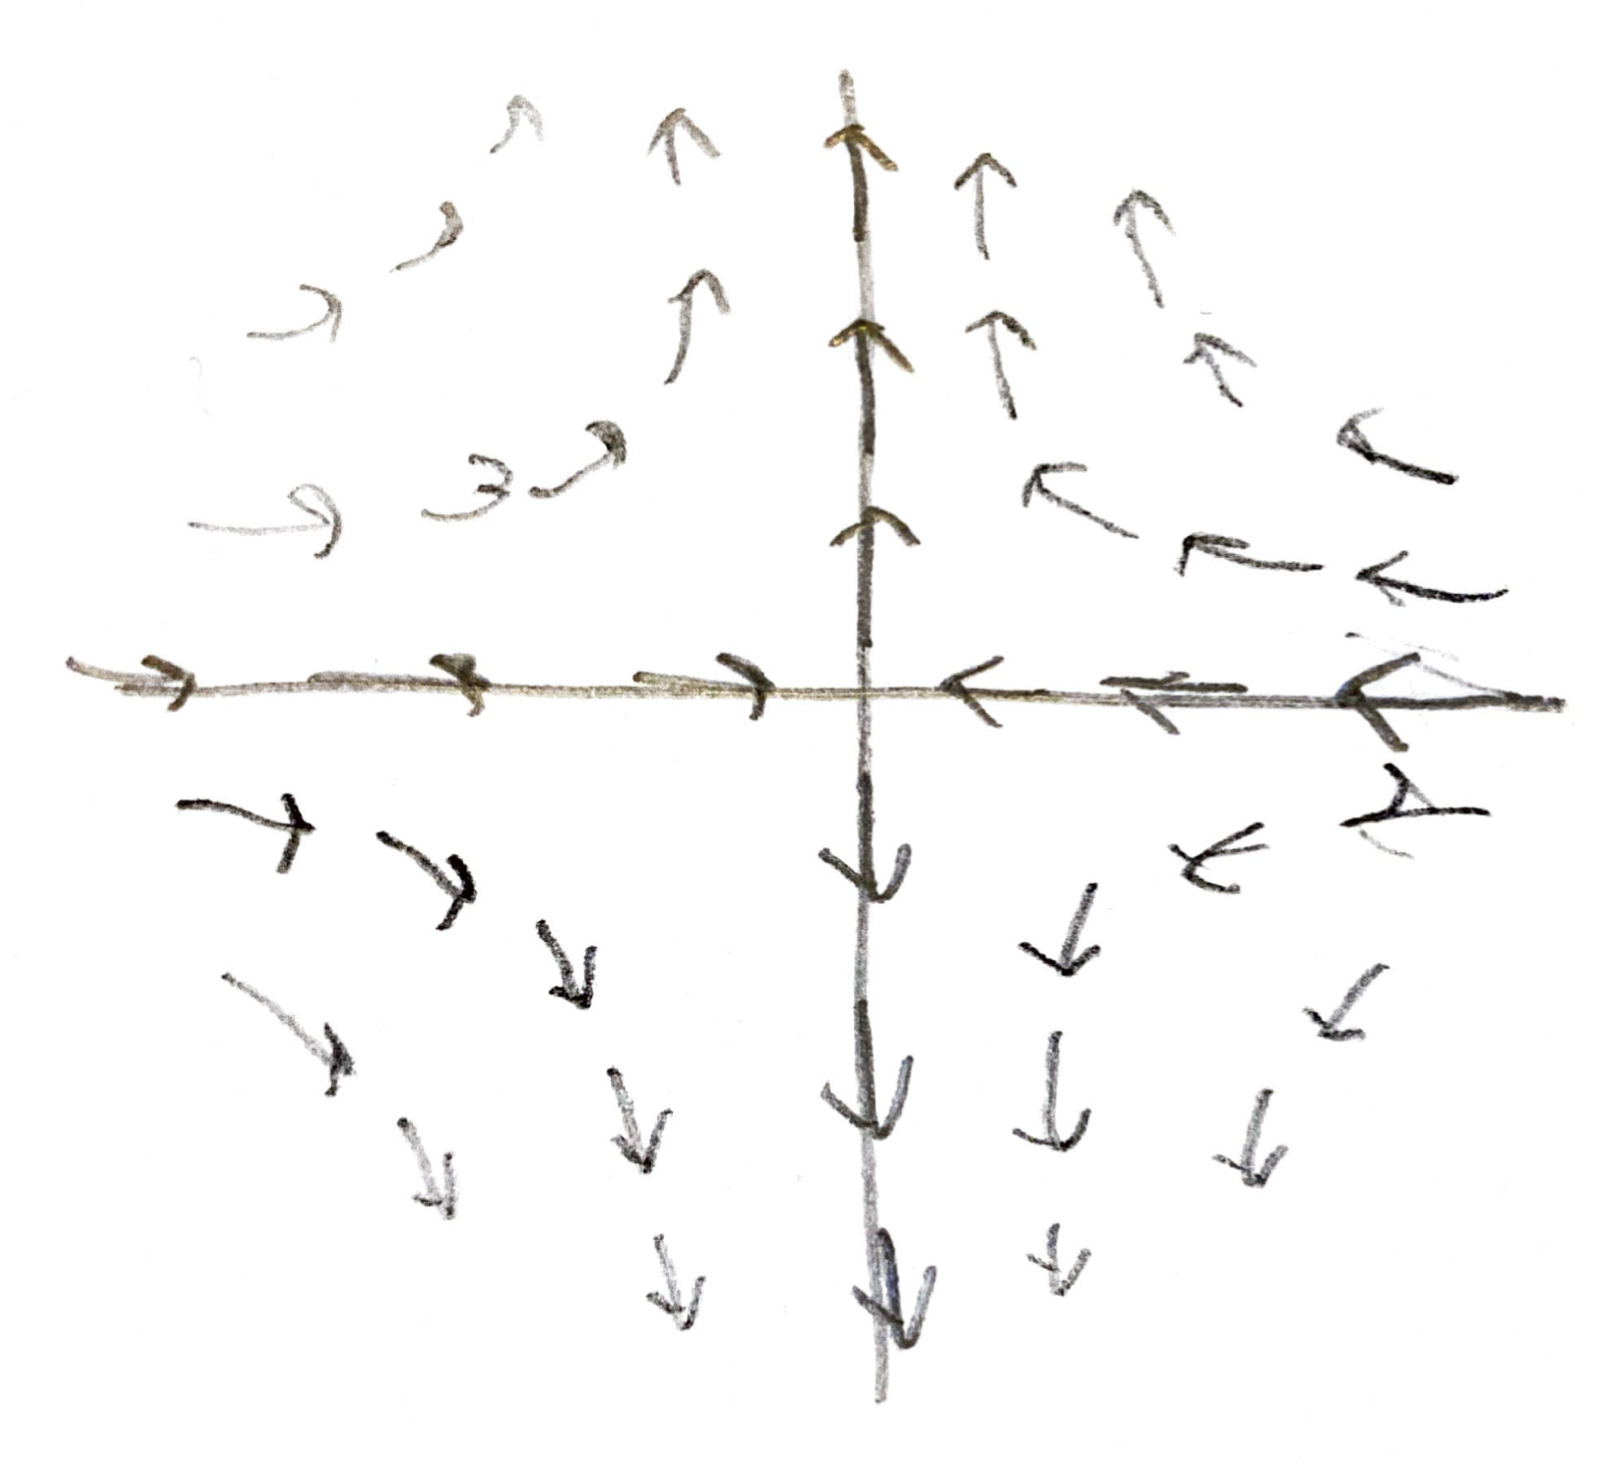
\includegraphics[width=0.4\linewidth]{../ExtFiles/pset7_1-2.png}
            \end{center}
        \end{proof}
    \end{enumerate}
    \item We did not provide any grant on stability of a fixed point of an autonomous system if the linearization at that point has purely imaginary eigenvalues. This exercise gives several examples with more details. As per the Canvas announcement, skip (1)-(2) and only do (3), but also discuss therein the case $\mu<0$ there now.
    \begin{enumerate}
        % \item Show that the fixed point $(0,0)$ of the systems
        % \begin{align*}
        %     \begin{pmatrix}
        %         x\\
        %         y\\
        %     \end{pmatrix}'
        %     &=
        %     \begin{pmatrix}
        %         -x^2\\
        %         -y^2\\
        %     \end{pmatrix}&
        %     \begin{pmatrix}
        %         x\\
        %         y\\
        %     \end{pmatrix}'
        %     &=
        %     \begin{pmatrix}
        %         x^2\\
        %         y^2\\
        %     \end{pmatrix}
        % \end{align*}
        % are respectively asymptotically stable/completely unstable.
        % \begin{proof}
        %     \underline{Left ODE:} We can solve componentwise to get
        %     \begin{equation*}
        %         \phi_t
        %         \begin{pmatrix}
        %             z\\
        %             w\\
        %         \end{pmatrix}
        %         =
        %         \begin{pmatrix}
        %             \frac{z}{1+tz}\\
        %             \frac{w}{1+tw}\\
        %         \end{pmatrix}
        %     \end{equation*}
        %     Now let $(z,w)^T\in\R^2$ be arbitrary. Then as $t\to +\infty$, the denominator above will diverge to $\infty$ as well, meaning that each component overall converges to zero. Therefore, $\phi_t(z,w)^T\to 0$ as $t\to +\infty$, so 0 is asymptotically stable, as desired.\par
        %     \underline{Right ODE:} We can solve componentwise to get
        %     \begin{equation*}
        %         \phi_t
        %         \begin{pmatrix}
        %             z\\
        %             w\\
        %         \end{pmatrix}
        %         =
        %         \begin{pmatrix}
        %             \frac{z}{1-tz}\\
        %             \frac{w}{1-tw}\\
        %         \end{pmatrix}
        %     \end{equation*}
        %     This solution has finite lifespan $t\in[0,1/\max(z,w))$. As $t\to\max(z,w)$, at least one of $1-tz$ and $1-tw$ will approach zero, causing the overall term to diverge to $\infty$, meaning that 0 is completely unstable.
        % \end{proof}
        % \item Find the stable and unstable subsets of the planar system
        % \begin{equation*}
        %     \begin{pmatrix}
        %         x\\
        %         y\\
        %     \end{pmatrix}'
        %     =
        %     \begin{pmatrix}
        %         x^2\\
        %         -y^2\\
        %     \end{pmatrix}
        % \end{equation*}
        % \begin{proof}
        %     Combining out answers to the above, we have
        %     \begin{empheq}[box=\fbox]{align*}
        %         W_s(0) &= \spn
        %         \begin{pmatrix}
        %             0\\
        %             1\\
        %         \end{pmatrix}\\
        %         W_u(0) &= \R^2\setminus W_s(0)
        %     \end{empheq}
        %     since instability in either coordinate makes the whole thing unstable, whereas stability must apply to both coordinates.
        % \end{proof}
        \setcounter{enumii}{2}
        \item Fix $\mu>0$. Show that the fixed point $(0,0)$ of the system
        \begin{equation*}
            \begin{pmatrix}
                x\\
                y\\
            \end{pmatrix}'
            =
            \begin{pmatrix}
                y-\mu x(x^2+y^2)\\
                -x-\mu y(x^2+y^2)\\
            \end{pmatrix}
        \end{equation*}
        is globally asymptotically stable, no matter how small $\mu$ is; that is, every orbit is attracted to it. This shows that periodic solutions of the harmonic oscillator are not persisted under higher order perturbation. \emph{Hint}: Find out the differential equation satisfied by the polar coordinates of an orbit.
        \begin{proof}
            Let $r^2=x^2+y^2$ and $\tan(\theta)=y/x$. Then
            \begin{align*}
                2rr' &= 2xx'+2yy'\\
                r' &= \frac{xx'+yy'}{r}\\
                &= \frac{x[y-\mu x(x^2+y^2)]+y[-x-\mu y(x^2+y^2)]}{r}\\
                &= \frac{xy}{r}-\mu x^2r-\frac{xy}{r}-\mu y^2r\\
                &= -\mu r(x^2+y^2)\\
                &= -\mu r^3
            \end{align*}
            and
            \begin{align*}
                \sec^2\theta\cdot\theta' &= \frac{xy'-yx'}{x^2}\\
                \theta' &= \frac{xy'-yx'}{x^2}\cdot\cos^2\theta\\
                &= \frac{xy'-yx'}{x^2}\cdot\frac{x^2}{r^2}\\
                &= \frac{xy'-yx'}{r^2}\\
                &= \frac{x[-x-\mu y(x^2+y^2)]-y[y-\mu x(x^2+y^2)]}{r^2}\\
                &= -\frac{x^2}{r^2}-\mu xy-\frac{y^2}{r^2}+\mu xy\\
                &= -\frac{x^2+y^2}{r^2}\\
                &= -1
            \end{align*}
            Thus, we can transform the original equation to
            \begin{equation*}
                \begin{pmatrix}
                    r\\
                    \theta\\
                \end{pmatrix}'
                =
                \begin{pmatrix}
                    -\mu r^3\\
                    -1\\
                \end{pmatrix}
            \end{equation*}
            for $r\geq 0$ and $\theta\in\R$. Solving the componentwise separable ODEs, we can deduce that the flow is
            \begin{equation*}
                \phi_t
                \begin{pmatrix}
                    z\\
                    w\\
                \end{pmatrix}
                =
                \begin{pmatrix}
                    \sqrt{\frac{z^2}{1+2\mu z^2t}}\\
                    w-t\\
                \end{pmatrix}
            \end{equation*}
            Consequently, for arbitrary $\mu>0$ and $x=(z,w)^T\in\R^2$, the denominator $1+2\mu z^2t\to\infty$ as $t\to +\infty$. Therefore, $r\to 0$ as $t\to +\infty$, so since we're using polar coordinates, $\phi_t(x)\to 0$, as desired.\par
            On the other hand, let $\mu<0$ and $x=(z,w)^T\in\R^2$ be arbitrary. Then as $t\to -1/2\mu z^2$ (a positive quantity since $\mu<0$), the denominator $1+2\mu z^2t\to 0$. Therefore, the overall term and consequently $r$ blows up in finite time.
        \end{proof}
    \end{enumerate}
    \item Consider the Duffing equation
    \begin{equation*}
        x''+bx'-x+x^3 = 0
        ,\quad
        b>0
    \end{equation*}
    \begin{enumerate}
        \item Convert it to a first order autonomous system. Find an "energy function" of the system.
        \begin{proof}
            Let $y=x$ and $z=x'$. Then we have that
            \begin{equation*}
                \boxed{
                    {
                        \begin{pmatrix}
                            y\\
                            z\\
                        \end{pmatrix}
                    }' = {
                        \begin{pmatrix}
                            z\\
                            -bz+y-y^3\\
                        \end{pmatrix}
                    }
                }
            \end{equation*}
            We can derive an energy function as follows.
            \begin{align*}
                0 &= x''+bx'+\underbrace{x^3-x}_{U'(x)}\\
                &= x'x''+b|x'|^2+x'U'(x)\\
                &= \left( \frac{1}{2}(x')^2 \right)'+b|x'|^2+(U(x))'\\
                -b|x'|^2 &= \dv{t}(\frac{1}{2}(x')^2+U(x))
            \end{align*}
            Therefore, the energy function is constantly decreasing.
        \end{proof}
        \item There are three fixed points for the system in part (1). Determine the local behavior of the fixed points using the stable manifold theorem and Hartman linearization theorem.
        \begin{proof}
            The fixed points are
            \begin{align*}
                \begin{pmatrix}
                    -1\\
                    0\\
                \end{pmatrix}&&
                \begin{pmatrix}
                    0\\
                    0\\
                \end{pmatrix}&&
                \begin{pmatrix}
                    1\\
                    0\\
                \end{pmatrix}
            \end{align*}
            We first analyze them via the stable manifold theorem.\par
            The linearization of the system at $(0,0)^T$ is
            \begin{equation*}
                A =
                \begin{pmatrix}
                    0 & 1\\
                    1 & -b\\
                \end{pmatrix}
            \end{equation*}
            Taking the characteristic polynomial and calculating eigenvalues can be done as follows.
            \begin{align*}
                0 &= \chi_A(z)\\
                &= -z(-b-z)-1\\
                &= z^2+bz-1\\
                z &= \frac{-b\pm\sqrt{b^2+4}}{2}
            \end{align*}
            Thus, one eigenvalue is always greater than zero and one is always less than zero, so we never have purely imaginary eigenvalues. Thus, $(0,0)^T$ is hyperbolic for all $b>0$, and $\dim\mathbb{E}_s=\dim\mathbb{E}_u=1$. Therefore,
            \begin{equation*}
                \boxed{(0,0)^T\text{ is locally a saddle point for all }b>0.}
            \end{equation*}
            The linearization of the system at both of the other fixed points is
            \begin{equation*}
                B =
                \begin{pmatrix}
                    0 & 1\\
                    -2 & -b\\
                \end{pmatrix}
            \end{equation*}
            Characteristic polynomial and eigenvalues:
            \begin{align*}
                0 &= \chi_A(z)\\
                &= -z(-b-z)+2\\
                &= z^2+bz+2\\
                z &= \frac{-b\pm\sqrt{b^2-8}}{2}
            \end{align*}
            Thus, if $b<\sqrt{8}$, the eigenvalues are complex conjugates with negative real part and hence $(1,0)^T,(-1,0)^T$ are both similar to spiral sinks. If $b=\sqrt{8}$, there is only one eigenvalue ($-\sqrt{2}$) and only one eigenvector $(-\sqrt{2},2)$, so $B$ is not diagonalizable and hence $(1,0)^T,(-1,0)^T$ are similar to the distorted $y=x\pm x\log x$ form. If $b>\sqrt{8}$, then the eigenvalues are real and negative. Here, we have a case where the fixed point is hyperbolic, $\dim\mathbb{E}_s=2$, and $\dim\mathbb{E}_u=0$. Consequently, $(1,0)^T,(-1,0)^T$ are sinks in this case. Therefore,
            \begin{empheq}[box=\fbox]{align*}
                (1,0)^T,(-1,0)^T &\text{ are locally spiral sinks for all }0<b<\sqrt{2}\\
                (1,0)^T,(-1,0)^T &\text{ are locally similar to }x\pm x\log x\text{ for }b=\sqrt{2}\\
                (1,0)^T,(-1,0)^T &\text{ are locally sinks for all }b>\sqrt{2}
            \end{empheq}
            By the Hartman linearization theorem, we can further analyze every $b>0$ for $(0,0)^T$ and $b>\sqrt{2}$ for $(1,0)^T,(-1,0)^T$. Indeed, this theorem tells us that not only do smooth, tangent submanifolds exist of the above dimensions, but all orbits near the fixed point but not lying on one of the stable/unstable manifolds are slight distortions of the corresponding linearized cases analyzed in Lecture 5.1.
        \end{proof}
        \item Show that the global stable set of part (1) consists of two curves $C_1,C_2$, starting from the fixed point $(0,0)$ and symmetric with respect to that point, tending to infinity. Show that every point not lying on $C_1$ or $C_2$ will be attracted to one of the other two fixed points. You may use the phase portrait drawer (\href{https://www.wolframalpha.com/widgets/view.jsp?id=9298fea31cf266903b3df7174b95ddd7}{link}) to get some numerical inspiration.
        \begin{proof}
            
        \end{proof}
    \end{enumerate}
    \item Study the system
    \begin{equation*}
        \begin{pmatrix}
            x\\
            y\\
        \end{pmatrix}'
        =
        \begin{pmatrix}
            -x-y^2\\
            x^2+y\\
        \end{pmatrix}
    \end{equation*}
    according to the general steps mentioned in class. For your convenience, you may use the phase portrait drawer (same as above) to get some numerical inspiration for your conjectures.
    \begin{enumerate}
        \item Determine the fixed points of the system.
        \begin{proof}
            This is equivalent to solving the system of equations
            \begin{align*}
                -x-y^2 &= 0\\
                x^2+y &= 0
            \end{align*}
            Substitute $x=-y^2$ (from the first equation) into the second equation and solve for $y$:
            \begin{align*}
                0 &= y+y^4\\
                0 &= y(y^3+1)\\
                y &= 0,-1
            \end{align*}
            It follows from $x=-y^2$ that the corresponding values of $x$ are $0,-1$, respectively. Therefore, the fixed points are
            \begin{equation*}
                \boxed{
                    \begin{pmatrix}
                        0\\
                        0\\
                    \end{pmatrix},
                    \begin{pmatrix}
                        -1\\
                        -1\\
                    \end{pmatrix}
                }
            \end{equation*}
        \end{proof}
        \item Study the local behavior of the system at the fixed points: Stability, tangents of the stable and unstable manifolds. \emph{Hint}: One of the fixed points has purely imaginary eigenvalues, so nothing about stability can be said by linearization.
        \begin{proof}
            % So find the linearizations at all the fixed points, then determine the stable and unstable subspaces using the eigenvalues/eigenvectors? No need to derive the stable/unstable manifolds.


            The linearization of the system at $(0,0)^T$ is
            \begin{equation*}
                A =
                \begin{pmatrix}
                    -1 & 0\\
                    0 & 1\\
                \end{pmatrix}
            \end{equation*}
            Thus, the eigenvalues and eigenvectors are
            \begin{align*}
                \lambda_1 &= -1&
                    \lambda_2 &= 1\\
                v_1 &=
                \begin{pmatrix}
                    1\\
                    0\\
                \end{pmatrix}&
                    v_2 &=
                    \begin{pmatrix}
                        0\\
                        1\\
                    \end{pmatrix}
            \end{align*}
            It follows that $(0,0)^T$ is a hyperbolic fixed point. Consequently, by the stable manifold theorem, both the stable and the unstable manifolds are of dimension 1, but the former is tangent to the $x$-axis and the latter is tangent to the $y$-axis. Overall $(0,0)^T$ is a saddle point.\par
            The linearization of the system at $(-1,-1)^T$ is
            \begin{equation*}
                B =
                \begin{pmatrix}
                    -1 & 2\\
                    -2 & 1\\
                \end{pmatrix}
            \end{equation*}
            with corresponding eigenvalues $\lambda=\pm i\sqrt{3}$. Therefore, as per the hint, nothing about stability can be said by the linearization.
        \end{proof}
        \item In fact, this system admits implicit solutions of the form $F(x,y)=c$, where $F$ is a polynomial in $x,y$. Find a polynomial $F$ that meets this requirement, and show that the system has infinitely many periodic solutions.
        \begin{proof}
            We take
            \begin{align*}
                \frac{x'}{y'} &= \frac{-x-y^2}{x^2+y}\\
                (x^2+y)\dv{x}{t} &= (-x-y^2)\dv{y}{t}\\
                (\underbrace{x^2+y}_{\pdv*{F}{x}})\dv{x}{t}+(\underbrace{x+y^2}_{\pdv*{F}{y}})\dv{y}{t} &= 0
            \end{align*}
            Thus,
            \begin{align*}
                \pdv{F}{x} &= x^2+y\\
                F(x,y) &= \frac{1}{3}x^3+yx+g(y)\\
                \pdv{F}{y} &= x+\dv{g}{y}\\
                x+y^2 &= x+\dv{g}{y}\\
                g(y) &= \frac{1}{3}y^3+c
            \end{align*}
            so if we let
            \begin{equation*}
                \boxed{F(x,y) = \frac{1}{3}(x^3+y^3)+xy}
            \end{equation*}
            then $F(x,y)=c$ is a solution for all $c\in\R$. In particular, when $0<c<1/3$, a connected set of points satisfying $F(x,y)=c$ form an ellipse.
        \end{proof}
        \item Use the polynomial you find in part (3) to explicitly determine what the stable and unstable set should look like. \emph{Hint}: The vector field is symmetric with respect to the bisector of the 1st and 3rd quadrants, and as a result, the global stable and unstable set should coincide with each other.
        \begin{proof}
            hi
        \end{proof}
    \end{enumerate}
    \item State and prove a one-dimensional version of the Poincar\'{e}-Bendixson theorem.
    \item Suppose $f:\R\to\R$ is a smooth function and $f(0)=0$. Consider the autonomous system
    \begin{equation*}
        \begin{pmatrix}
            x\\
            y\\
        \end{pmatrix}'
        =
        \begin{pmatrix}
            xf(x^2+y^2)-y\\
            yf(x^2+y^2)+x\\
        \end{pmatrix}
    \end{equation*}
    \begin{enumerate}
        \item Find the differential equation satisfied by the polar coordinate representation $(r(t),\varphi(t))$ of the orbit.
        \begin{proof}
            We proceed analogously to Q2(3). Thus, we convert to polar coordinates via
            \begin{align*}
                r' &= \frac{xx'+yy'}{r}\\
                &= \frac{x[xf(x^2+y^2)-y]+y[yf(x^2+y^2)+x]}{r}\\
                &= \frac{x^2f(x^2+y^2)}{r}-\frac{xy}{r}+\frac{y^2f(x^2+y^2)}{r}+\frac{xy}{r}\\
                &= \frac{(x^2+y^2)f(x^2+y^2)}{r}\\
                &= rf(r^2)
            \end{align*}
            and
            \begin{align*}
                \theta' &= \frac{xy'-yx'}{r^2}\\
                &= \frac{x[yf(x^2+y^2)+x]-y[xf(x^2+y^2)-y]}{r^2}\\
                &= \frac{xyf(x^2+y^2)}{r^2}+\frac{x^2}{r^2}-\frac{xyf(x^2+y^2)}{r^2}+\frac{y^2}{r^2}\\
                &= \frac{x^2+y^2}{r^2}\\
                &= 1
            \end{align*}
            This yields as our final answer
            \begin{equation*}
                \boxed{
                    {
                        \begin{pmatrix}
                            r\\
                            \theta\\
                        \end{pmatrix}'
                        =
                        \begin{pmatrix}
                            rf(r^2)\\
                            1\\
                        \end{pmatrix}
                    }
                }
            \end{equation*}
        \end{proof}
        \item Prove that if $p_0>0$ is an isolated zero of $f$, then the circle $r=\sqrt{p_0}$ is a limit cycle of the system. What if the zero is not isolated?
        \begin{proof}
            A limit cycle is a periodic orbit. Let $x=(\sqrt{p_0},\theta)$ be some point lying on the described circle. Then by part (1), $r'(x)=0$ and $\theta'(x)=1$. Thus, the integral curve at $x$ is the described circle. Depending on the specific nature of $f$, the circle can be either an attracting or repelling limit cycle for spirals both inside and outside.\par
            If the zero is not isolated, then we have a dense region (an annulus, actually) of concentric circle, each of which is a limit cycle and a self-contained, nonintersecting periodic orbit.
        \end{proof}
        \item Give an example of a planar system with infinitely many limit cycles. The famous Hilbert's 16th problem asks how many limit cycles there could be for a planar autonomous system of polynomial entries. The problem is unsolved even for quadratic polynomials: It is known that the number can be 0, 1, 2, 3, 4, but it is not known whether the number has an upper bound or not. Hence, your answer cannot be a polynomial system.
        \begin{proof}
            We could choose
            \begin{equation*}
                \boxed{
                    {
                        \begin{pmatrix}
                            r\\
                            \theta\\
                        \end{pmatrix}'
                        =
                        \begin{pmatrix}
                            \sin(r)\\
                            1\\
                        \end{pmatrix}
                    }
                }
            \end{equation*}
            Then we have circular limit cycles of every radius $r$ satisfying $\sin(r)=0$. Explicitly, we have limit cycle circles of radius
            \begin{equation*}
                r = \pi n
                ,\quad
                n\in\N_0
            \end{equation*}
            For all values $r$ at which $r''<0$, we have an attracting limit cycle. This is because in this case, at values slightly greater than $r$ we have $r'<0$ so that the flow gets pulled in, and at values slightly less than $r$ we have $r'>0$ so that the flow gets pushed out. It will be the other way around for all values of $r$ at which $r''>0$, i.e., we have a repelling limit cycles at these values.
        \end{proof}
    \end{enumerate}
\end{enumerate}


\subsection*{Study of Chemical Reactions}
In this section, you will explore how ordinary differential equations can be used to study long-term behavior of some chemical reactions.
\begin{enumerate}
    \item \textbf{Enzyme kinetics.} Consider an enzyme-catalyzed chemical reaction
    \begin{equation*}
        \ce{E + S <=>[$k_1$][$k_{-1}$] ES ->[$k_2$] E + P}
    \end{equation*}
    Here $k_1,k_2,k_{-1}$ are rate constants, which are positive. The materials involved in this reaction include the substrate \ce{S}, the enzyme \ce{E}, the enzyme-substrate complex \ce{ES}, and the final product \ce{P}. The concentrations of these materials (unit: mole per unit volume) satisfy the differential system
    \begin{align*}
        \dv{\cnc{S}}{t} &= -k_1\cnc{E}\cnc{S}+k_{-1}\cnc{ES}\\
        \dv{\cnc{E}}{t} &= -k_1\cnc{E}\cnc{S}+(k_{-1}+k_2)\cnc{ES}\\
        \dv{\cnc{ES}}{t} &= k_1\cnc{E}\cnc{S}-(k_{-1}+k_2)\cnc{ES}\\
        \dv{\cnc{P}}{t} &= k_2\cnc{ES}
    \end{align*}
    \begin{enumerate}
        \item Let $\cnc[0]{S}$ and $\cnc[0]{E}$ denote the initial concentrations of the substrate and enzyme, respectively. Find two first integrals for this system, and transform it into a 2D autonomous system in $x=\cnc{S}$ and $y=\cnc{ES}$. \emph{Hint}: Use the law of conservation of mass. The substrate is either transformed into product or the \ce{ES} complex and cannot just disappear, and the same reasoning applies for the enzyme. These two facts are reflected as some algebraic properties of the system.
        \begin{proof}
            By adding the second and third equations together, we get
            \begin{equation*}
                \dv{\cnc{E}}{t}+\dv{\cnc{ES}}{t} = 0
            \end{equation*}
            from which we obtain the first integral
            \begin{equation*}
                \cnc{E}+\cnc{ES} = c
            \end{equation*}
            for some $c\in\R$. In particular, this equation implies that the sum of the concentrations of the enzyme and enzyme-substrate complex is constant for all time, which makes sense since the enzyme must be in one of these two forms and cannot appear or disappear as per the law of conservation of mass. Now we determine the value of $c$. If this equation is valid for all time, it is valid specifically for $t=0$, when $\cnc{E}=\cnc[0]{E}$ and $\cnc{ES}=0$. Thus, $c=\cnc[0]{E}+0=\cnc[0]{E}$, and one of the first integrals is
            \begin{equation*}
                \boxed{\cnc{E}+\cnc{ES} = \cnc[0]{E}}
            \end{equation*}
            We can similarly determine by adding the first, third, and fourth equations together that the other first integral is
            \begin{equation*}
                \boxed{\cnc{S}+\cnc{ES}+\cnc{P} = \cnc[0]{S}}
            \end{equation*}
            Note that this also makes sense chemically as it corresponds to the conservation of the compound on which the enzyme acts in all of its forms.\par
            It follows that we can express $\dv*{\cnc{S}}{t},\dv*{\cnc{ES}}{t}$ in terms of only $\cnc{S},\cnc{ES}$ by substituting for $\cnc{E}$ using the first integrals. In particular, we may write
            \begin{align*}
                \dv{\cnc{S}}{t} &= -k_1(\cnc[0]{E}-\cnc{ES})\cnc{S}+k_{-1}\cnc{ES}\\
                \dv{\cnc{ES}}{t} &= k_1(\cnc[0]{E}-\cnc{ES})\cnc{S}-(k_{-1}+k_2)\cnc{ES}
            \end{align*}
            Note that these two ODEs capture all information in the system because the others can be derived from them using the derivatives of the first integrals. For example, the expression
            \begin{equation*}
                \dv{\cnc{E}}{t}+\dv{\cnc{ES}}{t} = 0
                \quad\Longleftrightarrow\quad
                \dv{\cnc{E}}{t} = -\dv{\cnc{ES}}{t}
            \end{equation*}
            Lastly, for the sake of simplicity, we can relabel $x=\cnc{S}$ and $y=\cnc{ES}$.
            \begin{empheq}[box=\fbox]{align*}
                \dv{x}{t} &= -k_1(\cnc[0]{E}-y)x+k_{-1}y\\
                \dv{y}{t} &= k_1(\cnc[0]{E}-y)x-(k_{-1}+k_2)y
            \end{empheq}
        \end{proof}
        \item There is only one fixed point of the system obtained in part (1). Study the stability of that fixed point.
        \begin{proof}
            We assume $\cnc[0]{E}>0$ (otherwise, every point is a fixed point). Under this assumption, the sole fixed point is
            \begin{equation*}
                \begin{pmatrix}
                    0\\
                    0\\
                \end{pmatrix}
            \end{equation*}
            The linearization at $(0,0)^T$ is
            \begin{equation*}
                A =
                \begin{pmatrix}
                    -k_1\cnc[0]{E} & k_{-1}\\
                    k_1\cnc[0]{E} & -(k_{-1}+k_2)\\
                \end{pmatrix}
            \end{equation*}
            yielding eigenvalues
            \begin{align*}
                0 &= \chi_A(z)\\
                &= (-k_1\cnc[0]{E}-z)(-(k_{-1}+k_2)-z)-k_{-1}k_1\cnc[0]{E}\\
                &= z^2+(k_1\cnc[0]{E}+k_{-1}+k_2)z+k_1\cnc[0]{E}(k_{-1}+k_2)-k_1k_{-1}\cnc[0]{E}\\
                &= z^2+(k_1\cnc[0]{E}+k_{-1}+k_2)z+k_1k_2\cnc[0]{E}\\
                z &= \frac{-(k_1\cnc[0]{E}+k_{-1}+k_2)\pm\sqrt{(k_1\cnc[0]{E}+k_{-1}+k_2)^2-4k_1k_2\cnc[0]{E}}}{2}
            \end{align*}
            It follows that both eigenvalues are negative and hence $(0,0)^T$ is a hyperbolic fixed point. In this case, $(0,0)^T$ is a sink (i.e., is \fbox{asymptotically stable}).
        \end{proof}
        \item Prove that any orbit starting from the first quadrant will stay in that quadrant, and will finally be attracted to the fixed point. What is the chemical explanation for this mathematical fact?
        \begin{proof}
            Consider the points along the $x$- and $y$-axes. For the points along the $x$-axis, we have $y=0$ and thus
            \begin{align*}
                \dv{x}{t} &= -k_1\cnc[0]{E}x\\
                \dv{y}{t} &= k_1\cnc[0]{E}x
            \end{align*}
            Importantly, the lower equation above implies that the vector field points inward toward first quadrant at every point along the $x$-axis.\par
            For the points along the $y$-axis, we have $x=0$ and thus
            \begin{align*}
                \dv{x}{t} &= k_{-1}y\\
                \dv{y}{t} &= -(k_{-1}+k_2)y
            \end{align*}
            Thus, similarly, the vector field points inward toward first quadrant at every point along the $y$-axis. Thus, by the proposition from Lecture 7.2, since $f(x)$ is transversal to the boundary and inward pointing, the set is invariant.
        \end{proof}
    \end{enumerate}
    \item \textbf{Iodine clock reaction.} Iodine clock reactions are perhaps the most interesting experiments to show to a beginner in chemistry. The chlorine dioxide-iodine-malonic acid (CDIMA) reaction is an example of one. Prepare a solution of chlorine dioxide, malonic acid, and starch. Then add in a solution of iodine. The color of the liquid will immediately turn to dark blue, and then the blue subsides to a light brown in a few seconds, and then it re-enters the blue-brown cycle. This process can last for nearly an hour. The blue color is due to the presence of a triiodine-starch complex, and the blue color subsides because the iodine is oxidized to the iodide ion. Thus, the change of color suggests the periodic oscillation of the concentration of iodine and the iodide ion. We shall give an explanation of this experimental fact using ODEs.\par
    In the Lengyel-Epstein model, the CDIMA reaction consists of three steps.
    \begin{align*}
        \ce{MA + I2} &\ce{->} \ce{IMA + I- + H+}\\
        \ce{ClO2 + I-} &\ce{->} \ce{ClO2- + \tfrac{1}{2}I2}\\
        \ce{ClO2- + 4I- + 4H+} &\ce{->} \ce{2I2 + Cl- + 2H2O}
    \end{align*}
    Here, MA stands for malonic acid \ce{CH(COOH)2} and IMA stands for iodomalonic acid \ce{CI(COOH)2}. According to the experiments of Lengyel, R\'{a}bai, and Epstein, the rates of these three reactions are, respectively,
    \begin{align*}
        r_1 &= \frac{k_{1a}\cnc{MA}\cnc{I2}}{k_{1b}+\cnc{I2}}\\
        r_2 &= k_2\cnc{ClO2}\cnc{I-}\\
        r_3 &= k_{3a}\cnc{ClO2-}\cnc{I-}\cnc{H+}+\frac{k_{3b}\cnc{ClO2-}\cnc{I2}\cnc{I-}}{u+\cnc{I-}^2}
    \end{align*}
    where $k_{1a},k_{1b},k_2,k_{3a},k_{3b},u$ are all constants. Lengyel, R\'{a}bai, and Epstein discovered that only the concentrations of the iodide ion and chloride ion change drastically, while the concentration of iodine and chlorine dioxide is approximately constant. So the change in concentration of the materials can be described by a 2D autonomous system
    \begin{align*}
        \dv{\cnc{I-}}{t} &= r_1-r_2'\cnc{I-}-\frac{4\tilde{r}_3\cnc{I-}\cnc{ClO2-}}{u+\cnc{I-}^2}\\
        \dv{\cnc{ClO2-}}{t} &= \tilde{r}_2\cnc{I-}-\frac{\tilde{r}_3\cnc{I-}\cnc{ClO2-}}{u+\cnc{I-}^2}
    \end{align*}
    where $\tilde{r}_2=k_2\cnc{ClO2}$ and $r_3=k_{3b}\cnc{I2}$. After suitable scaling, it is transformed to a dimensionless form
    \begin{align*}
        \dv{x}{t} &= a-x-\frac{4xy}{1+x^2}\\
        \dv{y}{t} &= b\left( x-\frac{xy}{1+x^2} \right)
    \end{align*}
    \begin{enumerate}
        \item Prove that the first quadrant is an invariant set. This makes sense since concentrations of chemical materials cannot be negative.
        \begin{proof}
            Consider the points along the $x$- and $y$-axes. For the points along the $x$-axis, we have $y=0$ and thus
            \begin{align*}
                \dv{x}{t} &= a-x\\
                \dv{y}{t} &= bx
            \end{align*}
            Importantly, the lower equation above implies that the vector field points inward toward first quadrant at every point along the $x$-axis.\par
            For the points along the $y$-axis, we have $x=0$ and thus
            \begin{align*}
                \dv{x}{t} &= a\\
                \dv{y}{t} &= 0
            \end{align*}
            Thus, similarly, the vector field points inward toward first quadrant at every point along the $y$-axis. Thus, by the proposition from Lecture 7.2, since $f(x)$ is transversal to the boundary and inward pointing, the set is invariant.
        \end{proof}
        \item The system has only one fixed point in the first quadrant. Find it.
        \begin{proof}
            We need to solve the system of equations
            \begin{align*}
                0 &= a-x-\frac{4xy}{1+x^2}\\
                0 &= b\left( x-\frac{xy}{1+x^2} \right)
            \end{align*}
            for $x,y\geq 0$. From the second equation, we get
            \begin{align*}
                \frac{xy}{1+x^2} &= x\\
                y &= 1+x^2
            \end{align*}
            Substituting into the first equation, we get
            \begin{align*}
                x+\frac{4xy}{y} &= a\\
                x+4x &= a\\
                x &= \frac{a}{5}
            \end{align*}
            Substituting back into $y=1+x^2$, we get
            \begin{equation*}
                y = 1+\frac{a^2}{25}
            \end{equation*}
            Therefore, the fixed point in the first quadrant is
            \begin{equation*}
                \boxed{\left( \frac{a}{5},1+\frac{a^2}{25} \right)}
            \end{equation*}
        \end{proof}
        \item Study the stability of the fixed point found in part (2). You should be able to derive an algebraic condition concerning $a,b$ such that the fixed point is asymptotically stable/completely unstable.
        \begin{proof}
            To begin, calculate the linearization of the system at the fixed point. Indeed, we have
            \begin{align*}
                A &= f'\left( \frac{a}{5},1+\frac{a^2}{25} \right)\\
                &=
                \begin{pmatrix}
                    \eval{\pdv{x}(a-x-\frac{4xy}{1+x^2})}_{\left( \frac{a}{5},1+\frac{a^2}{25} \right)} & \eval{\pdv{y}(a-x-\frac{4xy}{1+x^2})}_{\left( \frac{a}{5},1+\frac{a^2}{25} \right)}\\
                    \eval{\pdv{x}(b\left( x-\frac{xy}{1+x^2} \right))}_{\left( \frac{a}{5},1+\frac{a^2}{25} \right)} & \eval{\pdv{y}(b\left( x-\frac{xy}{1+x^2} \right))}_{\left( \frac{a}{5},1+\frac{a^2}{25} \right)}\\
                \end{pmatrix}\\
                &=
                \begin{pmatrix}
                    \eval{\left( -1-\frac{4y(1-x^2)}{(1+x^2)^2} \right)}_{\left( \frac{a}{5},1+\frac{a^2}{25} \right)} & \eval{\left( -\frac{4x}{1+x^2} \right)}_{\left( \frac{a}{5},1+\frac{a^2}{25} \right)}\\
                    \eval{b\left( 1-\frac{y(1-x^2)}{(1+x^2)^2} \right)}_{\left( \frac{a}{5},1+\frac{a^2}{25} \right)} & \eval{-\frac{bx}{1+x^2}}_{\left( \frac{a}{5},1+\frac{a^2}{25} \right)}\\
                \end{pmatrix}\\
                % &=
                % \begin{pmatrix}
                %     -1-\frac{4(1-a^2/25)}{1+a^2/25} & -\frac{4a/5}{1+a^2/25}\\
                %     b\left( 1-\frac{1-a^2/25}{1+a^2/25} \right) & -\frac{ab/25}{1+a^2/25}\\
                % \end{pmatrix}
                &=
                \begin{pmatrix}
                    -1-\frac{4(25-a^2)}{25+a^2} & -\frac{20a}{25+a^2}\\
                    b-b\frac{25-a^2}{25+a^2} & -\frac{5ab}{25+a^2}\\
                \end{pmatrix}
            \end{align*}
            Thus,
            \begin{align*}
                0 &= \chi_A(z)\\
                &= \frac{1}{(25+a^2)^2}\left( a^4z^2-3a^4z+5a^3bz+25a^3b+50a^2z^2+50a^2z+125abz+625ab+625z^2+3125z \right)\\
                % &= \frac{1}{(25+a^2)^2}\left[ (a^4+50a^2+625)z^2+(-3a^4+5a^3b+50a^2+125ab+3125)z+25a^3b+625ab \right]\\
                0 &= \left[ (25+a^2)^2z^2+(-3a^4+5a^3b+50a^2+125ab+3125)z+25a^3b+625ab \right]
            \end{align*}
            Applying the quadratic formula to the above equation will yield the desired result (when the roots are less than zero, we get stability, and greater than zero implies instability).
        \end{proof}
        \item Find a bounded invariant subset containing the fixed point you found in part (2).
        \begin{proof}
            Since everything will turn in towards the fixed center, we can just choose
            \begin{equation*}
                \overline{B\left( \left( \frac{a}{5},1+\frac{a^2}{25} \right),a/10 \right)}
            \end{equation*}
        \end{proof}
        \item Use the Poincar\'{e}-Bendixson theorem to prove that when the fixed point is completely unstable, the bounded invariant subset in part (4) contains at least one limit cycle. What is the implication in chemistry of this mathematical fact?
        \begin{proof}
            Let $\Omega$ denote the set from part (4). By the Poincar\'{e}-Bendixson theorem, $\omega(x)\subset\Omega$ is either a fixed point, a limit cycle, or consists of finitely many fixed points. If the fixed point is completely unstable, then it will lie in $\alpha(x)$, but $\omega(x)$ will be empty unless $x$ is the fixed point we've been working with, so it is not case 1. Since there is only one fixed point (as per part 2), we know it is not the third case either. Therefore, we must have the second case ($\omega(x)$ is a limit cycle), as desired.\par
            The implication in chemistry is that if we set up our system such that $a,b$ make the fixed point completely unstable, then $x,y$ (concentrations) will alternate periodically.
        \end{proof}
    \end{enumerate}
\end{enumerate}




\end{document}